\section{Case 2: Kompromitterte brukerkontoer ved NTNU}
\label{sec:case_kontoer}
NTNU er et stort universitet med mange ansatte. NTNU er derfor et mål for aktører med ondsinnede hensikter. En av disse hensiktene er å få tilgang til brukerkontoer. Disse kontoene blir brukt til mye forskjellig. De brukes ofte for spam, innhenting av store mengder forskningsartikler og videre salg. Måten disse kontoene kommer på avveie er uvisst, men noen av hypotesene innebærer phishing og gjenbruk av brukernavn og passord på nettsider som har blitt kompromittert. Vår oppgave i dette caset er å bruke rotårsaksanalyse til å finne og presentere tiltak som eliminerer rotårsaken til at kontoer ved NTNU blir kompromittert.

\subsubsection{Oversikt over oppgaven}
I 2017 var kompromitterte kontoer alene årsaken til omtrent 70 sikkerhetshendelser ved NTNU. NTNU har siden 2005 fått 5415 kontoer kompromittert. Disse kontoene ble funnet i en stor datadump i desember 2017. Av disse 5415 kontoene var 101 av dem fremdeles aktive. Det vil si at brukernavn og passord fortsatt var gyldige innloggingskredentialer da de ble avdekket. 

Universitetet kjenner bare årsakene til kompromitteringene i 5 av tilfellene. Phishing sto for fire og spam for en av hendelsene. 

\begin{figure}[H]
    \centering
    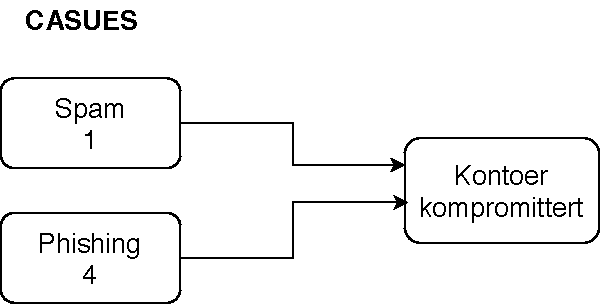
\includegraphics[scale=0.6]{case_2/bilder/kjente_arsaker.pdf}
    \caption[Kjente årsaker til kompromittert konto]{Kjente årsaker til kompromittert konto}
    \label{fig:kjente-arsaker-kompromittert-konto}
\end{figure}

Phishing er en av de få årsakene vi har data på, så det er en av årsakene vi vil holde fokus på i analysen. Bildet under viser eksempler på phishing e-post som har blitt sendt til ansatte ved NTNU.

\begin{figure}[H]%
    \centering
    \subfloat[Forsøk fra November 2017]{{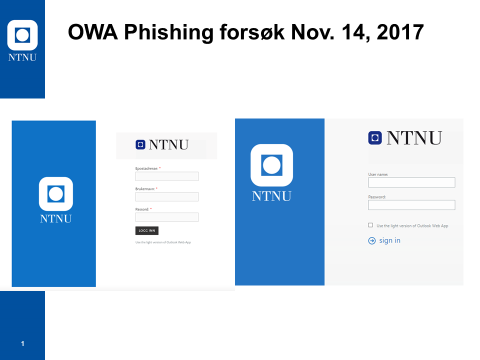
\includegraphics[width=5cm]{case_2/bilder/phishing_1.png} }}%
    \qquad
    \subfloat[Forsøk fra Januar 2018]{{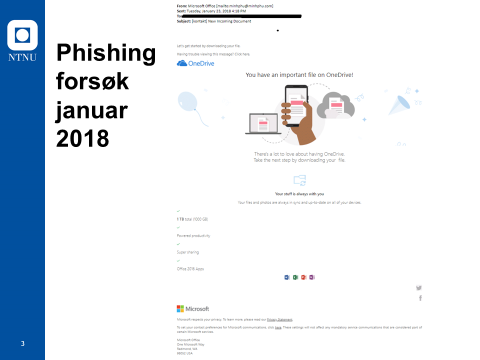
\includegraphics[width=5cm]{case_2/bilder/phishing_2.png} }}%
    \qquad
    \subfloat[Forsøk fra Januar 2018]{{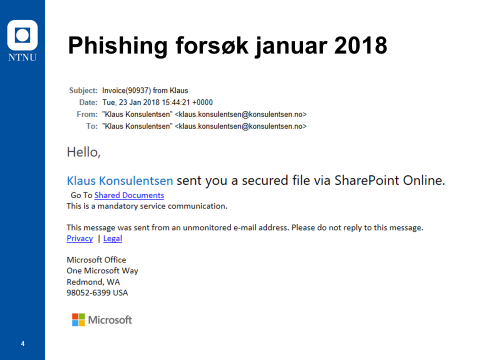
\includegraphics[width=5cm]{case_2/bilder/phishing_3.png} }}%
    \caption[Eksempel på phishing e-post]{Eksempel på phishing e-post som ble identifisert ved NTNU}%
    \label{fig:example}%
\end{figure}

Universitetet betaler for tilgang til databaser som inneholder tusenvis av forskningsartikler. 26 av de kompromitterte brukerne ble brukt av utenlandske aktører for å skaffe seg tilgang til forskningsartikler. Konsekvensen ved å ha kompromitterte kontoer som laster ned forskningsartikler er at NTNU risikerer å bli blokkert fra databasene. Angriperne derimot tjener på å ikke trenge å betale for tilgang til databasene. Det blir hentet ut flere tusen forskningsartikler per kompromitterte bruker. Universitetet vet ikke når det blir hentet ut artikler, eller om det er legitim bruk av artiklene. NTNU blir oppmerksom på problemet når de får beskjed fra samarbeidspartnere til NTNU, for eksempel de som tilbyr artikler. 

Et annet punkt som gjør det lukrativt å kompromittere universitetskontoer er at disse kontoene kan bli solgt på nett, der kredentialer behandles som ferskvare. \cite{PrisKonto}. 
\begin{figure}[H]
    \centering
    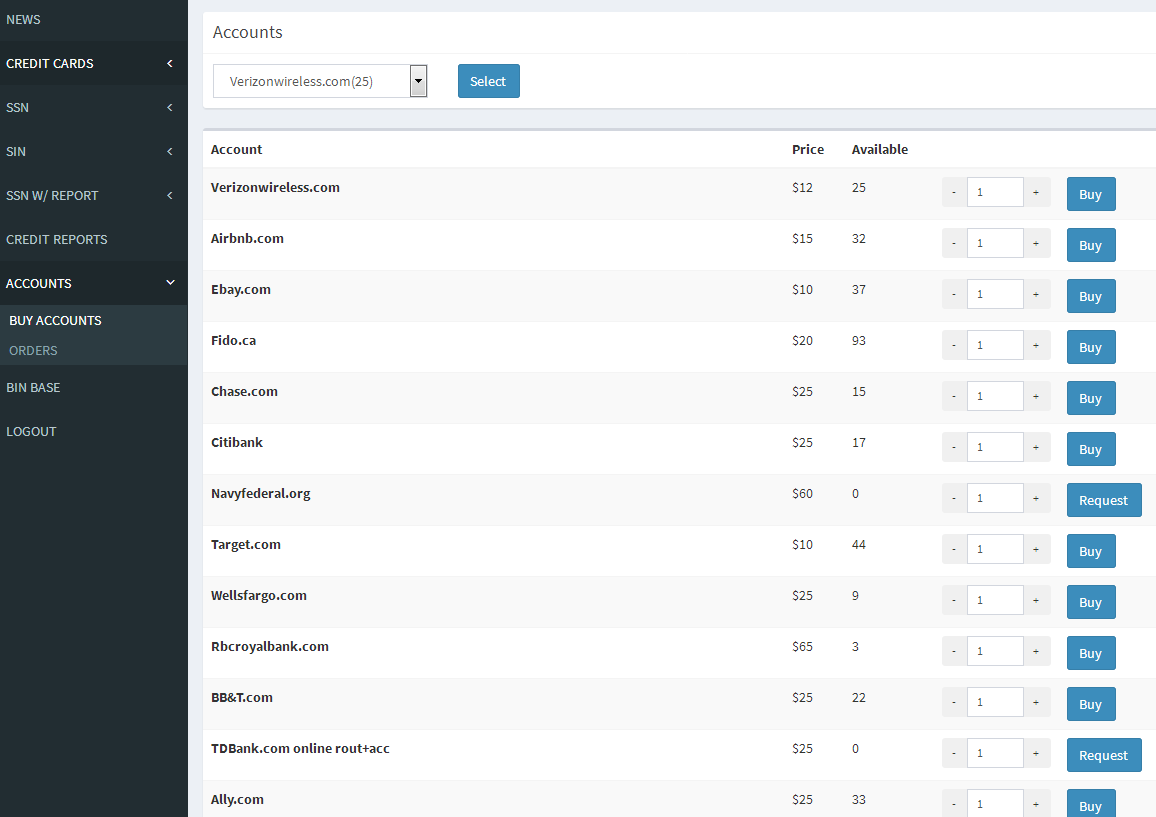
\includegraphics[scale=0.3]{case_2/bilder/prislite_kontore.png}
    \caption[Pris på kontoer]{Pris på kontoer}
    \label{fig:pris-kontoer}
\end{figure}

Figur \ref{fig:pris-kontoer} viser at det er et stort marked for brukerkontoer, og siden NTNU har mange samarbeidspartnere er de et stort mål for trusselaktørene. 

Denne analysen går ut på å identifisere rotårsaken til hvorfor NTNU har så mange kompromitterte brukerkontoer og komme med en tiltaksplan.